\documentclass{article}

\usepackage{textcomp}
\usepackage{fontenc}
\usepackage{graphicx}
\usepackage{caption}
\usepackage{gensymb} % for \degree
\usepackage{placeins} % for \images
\usepackage[margin=1in]{geometry} % to set margins
\usepackage{cite} % for bibtex


\renewcommand{\familydefault}{\sfdefault}
\graphicspath{{images/}}	% Root directory of the figures
\setlength{\parskip}{2 mm}

\usepackage{Sweave}
\begin{document}

\Sconcordance{concordance:SuppMat_Budburst.tex:SuppMat_Budburst.Rnw:%
1 16 1 1 0 29 1 1 13 1 45 38 0 1 2 1 24 24 0 1 2 1 7 24 0 1 3 84 1}
 % 

\flushleft

\textbf{\large{Supplemental Materials: Photoperiod and temperature interactively drive spring phenology in multiple species}}

Flynn, Wolkovich...

\textit{The Arnold Arboretum of Harvard University}

%% Add S prefix for tables and figures in Supplemental Materials
\renewcommand{\thetable}{S\arabic{table}}
\renewcommand{\thefigure}{S\arabic{figure}}

\section*{Literature Review}

We conducted a literature review, finding 109 studies which investigated effects of photoperiod, temperature, or their interaction on the timing of bud burst or flowering for woody or semi-woody plants.  No study varied chilling period, photoperiod, and temperature simultaneously across multiple species at multiple sites. Of those studies, eight simultaneously manipulated photoperiod and temperature. Basler \& Koerner \cite{Basler:2014aa} found a negative tradeoff between sensitivity to photoperiod and sensitivity to warming for four species, for example with \emph{Fagus sylvatica} advanced on average in leafout by 12 days in response to experimentally lengthened photoperiod, but only ca. 8 days in response to warmer temperatures, while \emph{Acer pseudoplatanus} advanced in leafout by 17 days in response to warming but essentially had no change in response to photoperiod. The current study expands on this work by including 28 species, across two sites, with addition manipulations of chilling temperature.

\section*{Chilling calculations}
The cuttings were harvested in late January 2015, and thus experienced substantial natural chilling by the time they were harvested. Using weather station data from the Harvard Forest and St. Hippolyte site, chilling hours (below 7.2\degree C), Utah Model chill portions (hours below 7.2\degree C and between 0\degree C and 7.2\degree C) and Dynamic Model \cite{Erez:1988} chill portions were calculated both for the natural chilling experienced by harvest and the chilling experienced in the 4\degree C and 1.5\degree C treatments. The Utah Model and Dynamic Model of chill portions account for variation in the amount of chilling accumulated at different temperatures, with the greatest chilling occurring approximately between 5-10\degree C, and fewer chill portions accumulating at low temperatures and that higher temperatures can reduce accumulated chilling effects. The two differ in the parameters used to determine the shape of the chilling accumulation curve, with the Dynamic Model being shown to be the most successful in predicting phenology for some woody species \cite{Luedeling:2009}.
With both the Utah and Dynamic model, the more severe chilling treatment resulted in fewer calculated chilling portions. 


%%%%%%%%%%%%%%%%%%%%%%%%%%%%%%%%%%%%
\section*{References Cited}
%%%%%%%%%%%%%%%%%%%%%%%%%%%%%%%%%%%%

\bibliography{danlib}
\bibliographystyle{naturemag}

%%%%%%%%%%%%%%%%%%%%%%%%%%%%%%%
\section*{Supplemental Figures and Tables}
%%%%%%%%%%%%%%%%%%%%%%%%%%%%%%%

% latex table generated in R 3.2.3 by xtable 1.8-2 package
% Mon Aug 22 13:01:01 2016
\begin{table}[ht]
\centering
\caption{Mean leafout and budburst days for the 28 species at both Harvard Forest, USA and St. Hippoltye, Canada} 
\begin{tabular}{lrrrr}
  \hline
Species & Budburst.HF & Budburst.SH & Leafout.HF & Leafout.SH \\ 
  \hline
\textit{Acer pensylvanicum} & 16.40 & 18.33 & 40.88 & 46.94 \\ 
  \textit{Acer rubrum} & 22.40 & 25.15 & 40.59 & 44.40 \\ 
  \textit{Acer saccharum} & 44.96 & 36.48 & 57.07 & 46.88 \\ 
  \textit{Alnus incana subsp. rugosa} & 32.91 & 25.36 & 45.15 & 44.36 \\ 
  \textit{Aronia melanocarpa} & 13.62 &  & 29.83 &  \\ 
  \textit{Betula alleghaniensis} & 19.67 & 20.77 & 33.51 & 34.64 \\ 
  \textit{Betula lenta} & 29.83 &  & 50.57 &  \\ 
  \textit{Betula papyrifera} & 16.89 & 18.04 & 28.71 & 35.63 \\ 
  \textit{Corylus cornuta} & 24.86 & 19.04 & 33.95 & 30.38 \\ 
  \textit{Fagus grandifolia} & 41.82 & 43.13 & 48.54 & 46.90 \\ 
  \textit{Fraxinus nigra} & 38.00 & 38.00 & 52.28 & 46.91 \\ 
  \textit{Hamamelis virginiana} & 43.67 &  & 47.38 &  \\ 
  \textit{Ilex mucronatus} & 15.80 & 15.49 & 26.97 & 25.15 \\ 
  \textit{Kalmia angustifolia} & 30.25 & 32.48 & 37.80 & 42.20 \\ 
  \textit{Lonicera canadensis} & 16.91 & 15.75 & 28.26 & 25.08 \\ 
  \textit{Lyonia ligustrina} & 30.87 &  & 49.50 &  \\ 
  \textit{Nyssa sylvatica} & 31.65 &  & 52.87 &  \\ 
  \textit{Populus grandidentata} & 33.43 & 31.23 & 46.21 & 45.17 \\ 
  \textit{Prunus pensylvanica} & 17.81 & 16.21 & 32.13 & 29.65 \\ 
  \textit{Quercus alba} & 45.23 &  & 52.91 &  \\ 
  \textit{Quercus rubra} & 36.43 & 33.57 & 45.02 & 42.80 \\ 
  \textit{Quercus velutina} & 52.09 &  & 59.16 &  \\ 
  \textit{Rhamnus frangula} & 32.38 &  & 37.29 &  \\ 
  \textit{Rhododendron prinophyllum} & 29.25 &  & 52.14 &  \\ 
  \textit{Spiraea alba} & 18.00 & 20.21 & 25.94 & 24.62 \\ 
  \textit{Vaccinium myrtilloides} & 13.12 & 17.27 & 27.00 & 28.95 \\ 
  \textit{Viburnum cassinoides} & 15.41 & 18.46 & 16.80 & 18.71 \\ 
  \textit{Viburnum lantanoides} & 31.25 & 27.54 & 32.02 & 26.41 \\ 
   \hline
\end{tabular}
\end{table}
% latex table generated in R 3.2.3 by xtable 1.8-2 package
% Mon Aug 22 13:01:01 2016
\begin{table}[ht]
\centering
\caption{Summary of mixed effect model of budburst day by species.} 
\begin{tabular}{rrrrrrr}
  \hline
 & mean & sd & 25\% & 50\% & 75\% & Rhat \\ 
  \hline
Temperature & -6.80 & 1.71 & -7.95 & -7.02 & -5.63 & 1.05 \\ 
  Photoperiod & -3.96 & 1.67 & -5.13 & -4.13 & -2.80 & 1.05 \\ 
  Chilling 4 \degree C & -22.09 & 2.84 & -24.05 & -21.75 & -20.26 & 1.03 \\ 
  Chilling 1.5 \degree C & -19.79 & 2.96 & -22.32 & -19.90 & -17.78 & 1.13 \\ 
  Site & 2.59 & 1.88 & 0.93 & 2.54 & 3.93 & 1.13 \\ 
  Temperature $\times$ Photoperiod & -0.60 & 0.72 & -1.07 & -0.46 & -0.24 & 1.02 \\ 
  Temperature $\times$ Site & 9.17 & 1.00 & 8.50 & 9.32 & 9.77 & 1.03 \\ 
  Photoperiod $\times$ Site & 9.68 & 1.06 & 9.11 & 9.57 & 10.33 & 1.00 \\ 
  Temperature $\times$ Chilling 4 \degree C & -0.18 & 0.96 & -0.82 & -0.06 & 0.47 & 1.04 \\ 
  Temperature $\times$ Chilling 1.5 \degree C & -0.02 & 1.03 & -0.67 & 0.14 & 0.48 & 1.02 \\ 
  Photoperiod $\times$ Chilling 4 \degree C & -1.48 & 0.76 & -1.99 & -1.35 & -1.00 & 1.04 \\ 
  Photoperiod $\times$ Chilling 1.5 \degree C & 0.05 & 0.79 & -0.52 & 0.09 & 0.76 & 1.10 \\ 
  Site $\times$ Chilling 4 \degree C & -1.96 & 1.33 & -2.84 & -1.86 & -0.85 & 1.09 \\ 
  Site $\times$ Chilling 1.5 \degree C & -3.49 & 1.23 & -4.14 & -3.55 & -2.78 & 1.01 \\ 
   \hline
\end{tabular}
\end{table}
% latex table generated in R 3.2.3 by xtable 1.8-2 package
% Mon Aug 22 13:01:01 2016
\begin{table}[ht]
\centering
\caption{Summary of mixed effect model of leafout day by species.} 
\begin{tabular}{rrrrrrr}
  \hline
 & mean & sd & 25\% & 50\% & 75\% & Rhat \\ 
  \hline
Temperature & -21.91 & 1.72 & -23.05 & -21.90 & -20.75 & 1.01 \\ 
  Photoperiod & -13.68 & 1.69 & -14.79 & -13.71 & -12.56 & 1.02 \\ 
  Chilling 4 \degree C & -26.37 & 3.09 & -28.41 & -26.41 & -24.41 & 1.01 \\ 
  Chilling 1.5 \degree C & -26.14 & 3.09 & -28.29 & -26.23 & -24.03 & 1.01 \\ 
  Site & 3.00 & 2.05 & 1.67 & 3.00 & 4.43 & 1.02 \\ 
  Temperature $\times$ Photoperiod & 3.54 & 0.77 & 2.99 & 3.54 & 4.07 & 1.02 \\ 
  Temperature $\times$ Site & 10.19 & 1.16 & 9.47 & 10.12 & 10.93 & 1.00 \\ 
  Photoperiod $\times$ Site & 11.29 & 1.25 & 10.44 & 11.26 & 12.09 & 1.01 \\ 
  Temperature $\times$ Chilling 4 \degree C & 0.77 & 1.05 & 0.08 & 0.79 & 1.48 & 1.00 \\ 
  Temperature $\times$ Chilling 1.5 \degree C & 2.41 & 1.27 & 1.60 & 2.41 & 3.24 & 1.01 \\ 
  Photoperiod $\times$ Chilling 4 \degree C & -0.59 & 0.82 & -1.11 & -0.58 & -0.04 & 1.03 \\ 
  Photoperiod $\times$ Chilling 1.5 \degree C & -1.00 & 0.83 & -1.55 & -1.01 & -0.42 & 1.02 \\ 
  Site $\times$ Chilling 4 \degree C & -1.87 & 1.26 & -2.67 & -1.92 & -1.05 & 1.01 \\ 
  Site $\times$ Chilling 1.5 \degree C & -3.46 & 1.38 & -4.39 & -3.44 & -2.52 & 1.01 \\ 
   \hline
\end{tabular}
\end{table}

% latex table generated in R 3.2.3 by xtable 1.8-2 package
% Mon Aug 22 13:01:01 2016
\begin{table}[ht]
\centering
\caption{Chill units in field and field and growth chamber conditions.} 
\begin{tabular}{llrrr}
  \hline
Site & Treatment & Chilling Hours & Utah Model & Chill portions \\ 
  \hline
Harvard Forest & Field chilling & 892 & 814.50 & 56.62 \\ 
   & 4.0 \degree C x 30 d & 2140 & 2062.50 & 94.06 \\ 
   & 1.5 \degree C x 30 d & 2140 & 1702.50 & 91.17 \\ 
  St. Hippolyte & Field chilling & 682 & 599.50 & 44.63 \\ 
   & 4.0 \degree C x 30 d & 1930 & 1847.50 & 82.06 \\ 
   & 1.5 \degree C x 30 d & 1930 & 1487.50 & 79.18 \\ 
   \hline
\end{tabular}
\end{table}
% latex table generated in R 3.2.3 by xtable 1.8-2 package
% Mon Aug 22 13:01:01 2016
\begin{table}[ht]
\centering
\caption{Phylogenetic signal in timing of bud burst and leaf out and species specific traits, as estimated in the caper package with simultaneous fitting of lambda.  Pore anatomy (ring- versus diffuse-porous species) was highly clustered phylogenetically, but no other trait examined demonstrated significant phylogenetic signal} 
\begin{tabular}{lr}
  \hline
Relationship & Lambda \\ 
  \hline
SLA - Temperature & 0.000 \\ 
  SLA - Photoperiod & 0.000 \\ 
  SLA - Chilling 4 \degree C & 0.000 \\ 
  SLA - Chilling 1.5 \degree C & 0.000 \\ 
  Wood Density - Temperature & 0.000 \\ 
  Wood Density - Photoperiod & 0.000 \\ 
  Wood Density - Chilling 4 \degree C & 0.000 \\ 
  Wood Density - Chilling 1.5 \degree C & 0.000 \\ 
  \% N - Temperature & 0.285 \\ 
  \% N - Photoperiod & 0.203 \\ 
  \% N - Chilling 4 \degree C & 0.127 \\ 
  \% N - Chilling 1.5 \degree C & 0.130 \\ 
  Pore anatomy - Temperature & 1.000 \\ 
  Pore anatomy - Photoperiod & 1.000 \\ 
  Pore anatomy - Chilling 4 \degree C & 1.000 \\ 
  Pore anatomy - Chilling 1.5 \degree C & 1.000 \\ 
   \hline
\end{tabular}
\end{table}
%% \clearpage % use if get 'too many unprocessed floats' error

\clearpage 

% Fig S1: Raw data plot

\begin{figure} 
\begin{center}
\caption{Coordinated responses of 28 woody plant species to photoperiod and temperature cues for leaf out. Color of circle reflect unmodeled data on average leaf out day across treatments, across sites of origin, while size of circle represents the total number of clippings in the experiment---this varies mainly based on whether the species was found at both sites and whether it was exposed to all three chilling treatments. } % Changed legend, check that I did it correctly please! Yes, ok.
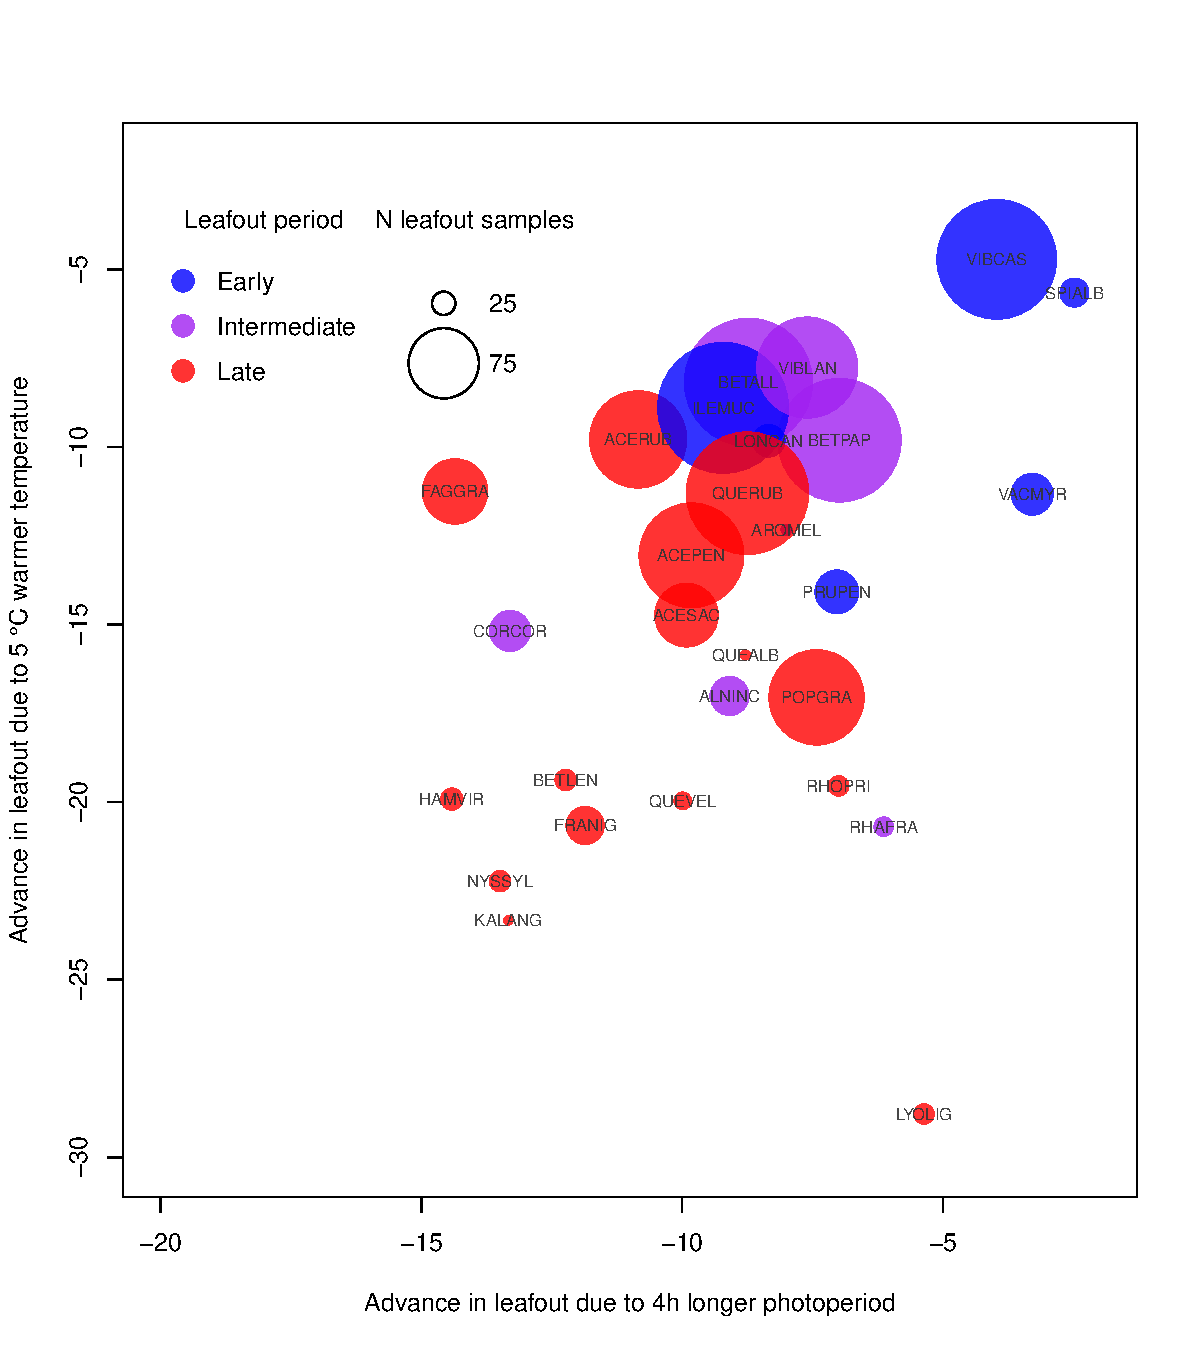
\includegraphics[scale=0.5]{Advplot2}
\label{fig1}
\end{center}
\end{figure}


\begin{figure}
\caption{Model estimates of effects of each predictors on bud burst, including species-level effects.}
\label{figS2}
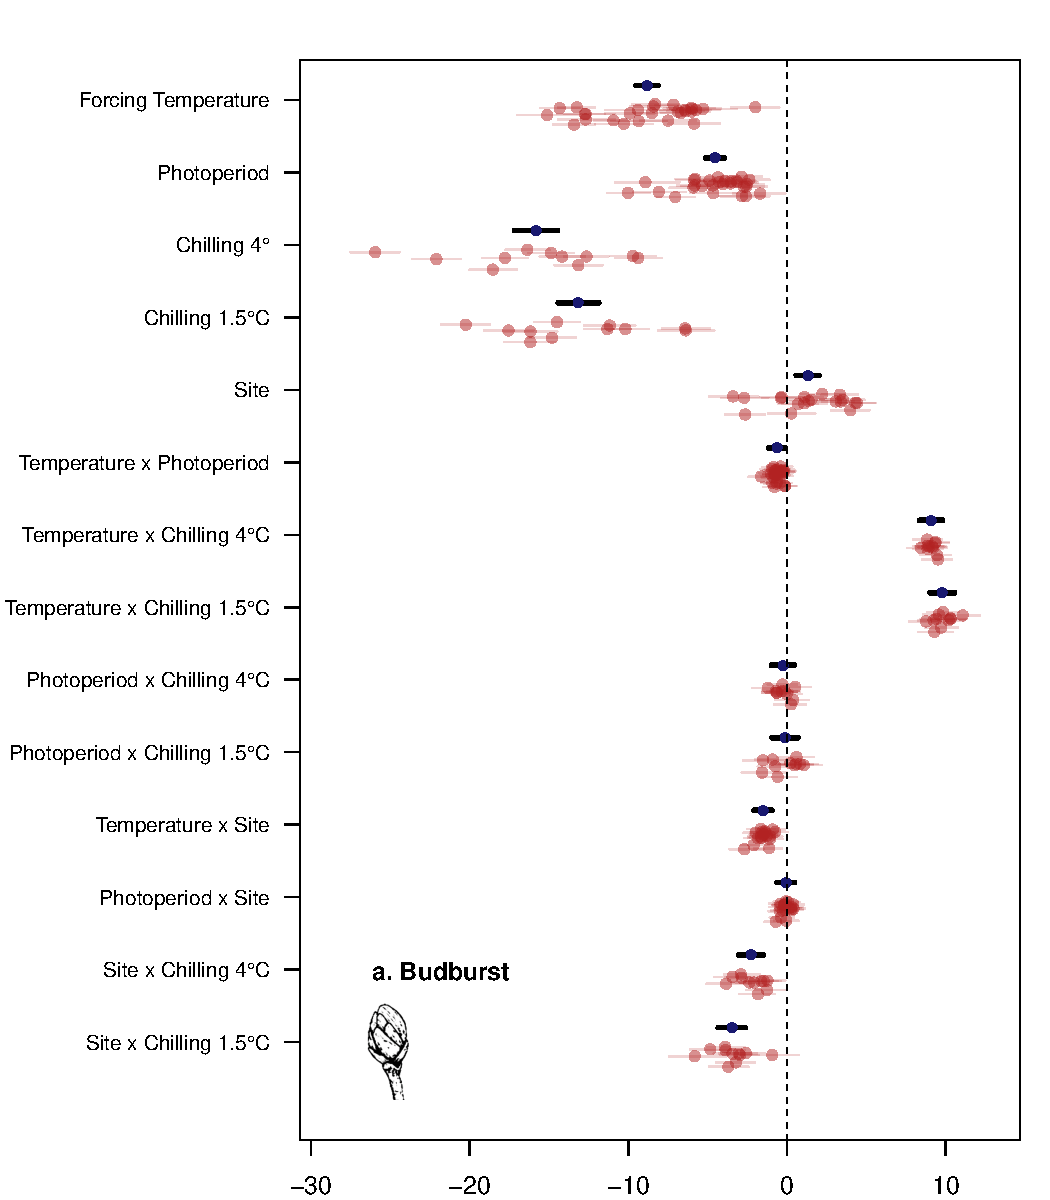
\includegraphics[scale=0.75, page=1]{Fig1_bb_lo+sp}
\end{figure}

\clearpage

\begin{figure}
\caption{Model estimates of leafout, including species-level effects.}
\label{figS3}
\includegraphics[scale=0.75, page=2]{Fig1_bb_lo+sp}
\end{figure}

\begin{figure}
\caption{Model estimates of sensitivity to warming, photoperiod, and chilling, compared to day of budburst (upper panels) or leafout (lower panels) across all experimental conditions.}
\label{figS4}
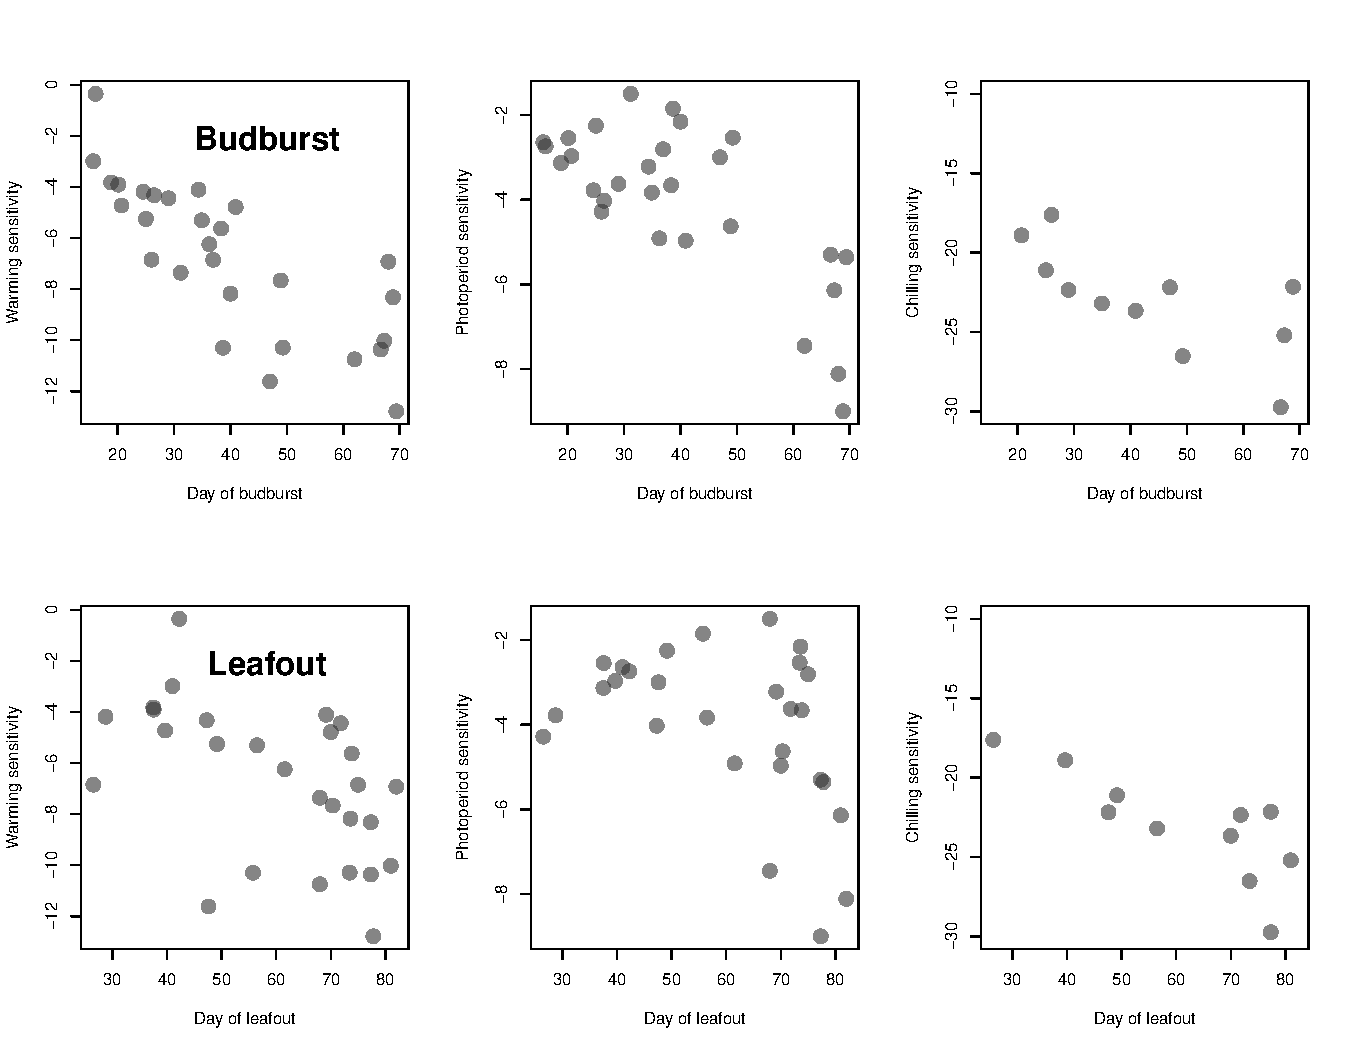
\includegraphics[scale=0.75]{Sens_vs_day}
\end{figure}

\clearpage

\begin{figure}
\caption{Trait sensitivity based on specific leaf area}
\label{figS5}
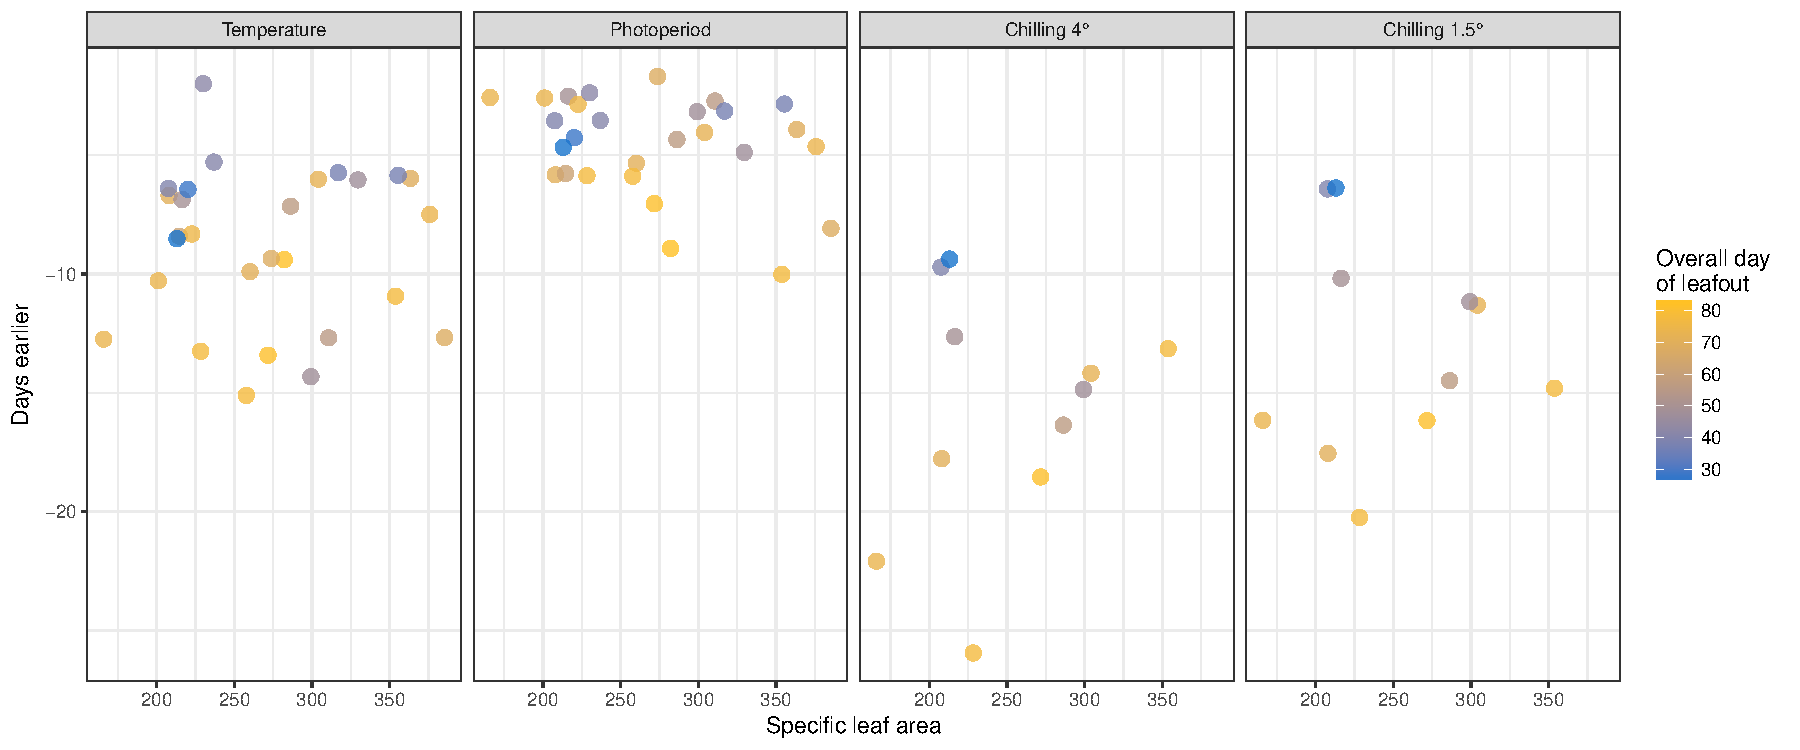
\includegraphics[scale=0.95, page=1]{Traits_vs_sensitivity}
\end{figure}

\begin{figure}
\caption{Trait sensitivity based on stem density}
\label{figS6}
\includegraphics[scale=0.95, page=2]{Traits_vs_sensitivity}
\end{figure}

\begin{figure}
\caption{Trait sensitivity based on \% nitrogen}
\label{figS7}
\includegraphics[scale=0.95, page=3]{Traits_vs_sensitivity}
\end{figure}


\begin{figure}
\caption{Specific leaf area and stem density by trees vs shrubs}
\label{figS8}
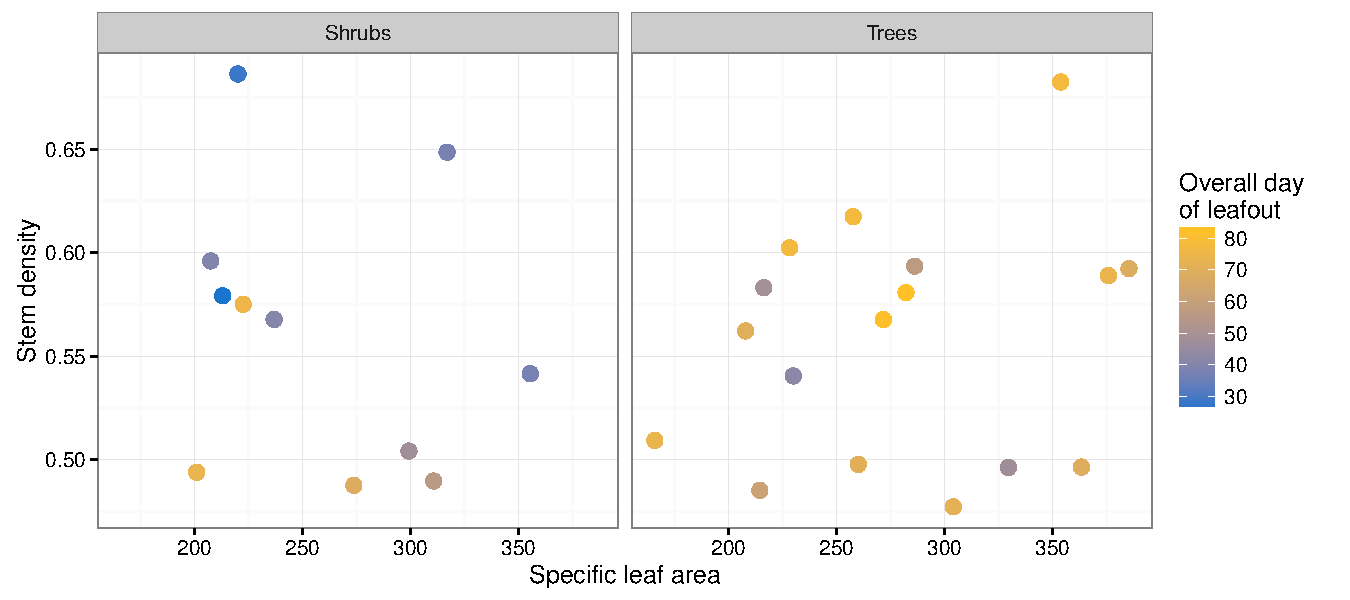
\includegraphics[scale=0.95, page=1]{Tree_shrub_traits}
\end{figure}


\begin{figure}
\caption{Specific leaf area and percent nitrogen by trees vs shrubs}
\label{figS9}
\includegraphics[scale=0.95, page=2]{Tree_shrub_traits}
\end{figure}

\begin{figure}
\caption{Stem density and percent nitrogen by trees vs shrubs}
\label{figS10}
\includegraphics[scale=0.95, page=3]{Tree_shrub_traits}
\end{figure}

\clearpage


\begin{figure}
\caption{Leafout rank order in experimental treatments vs. O'Keefe observations}
\label{figS11}
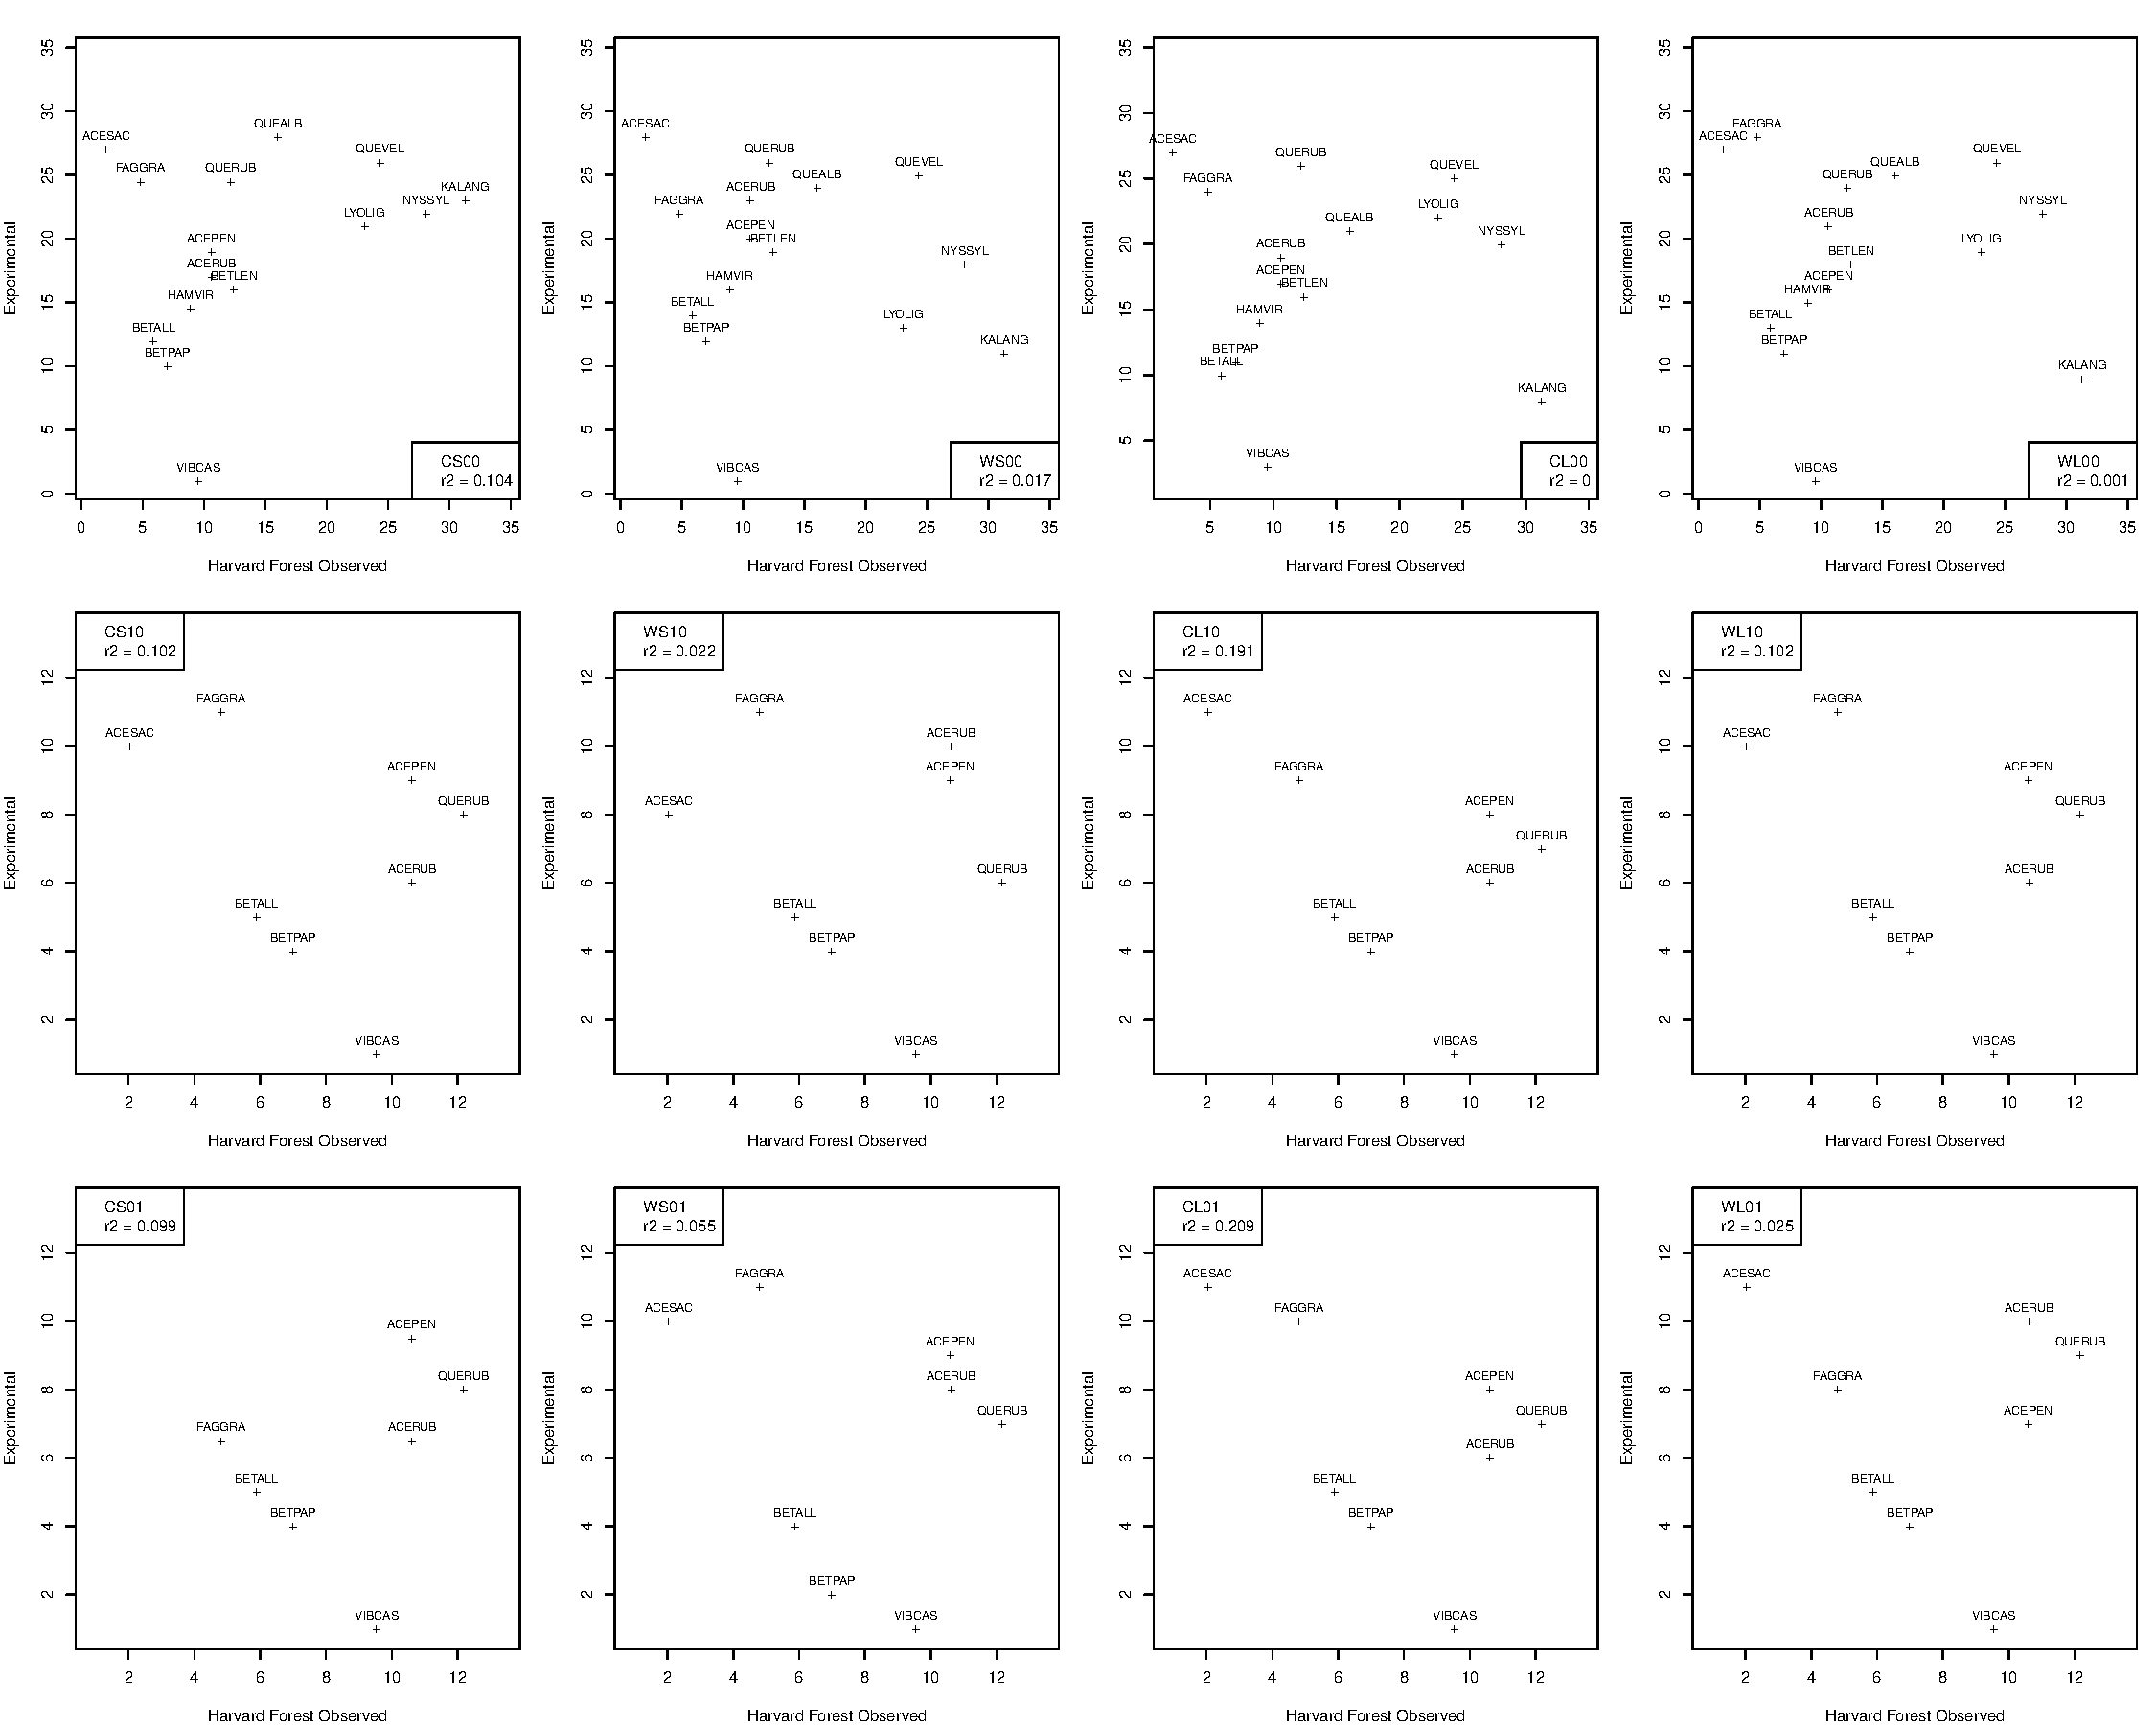
\includegraphics{leafout_exp_obs_corr}
\end{figure}

\begin{figure}
\caption{Leafout day of year in experimental treatments vs. O'Keefe observations}
\label{figS12}
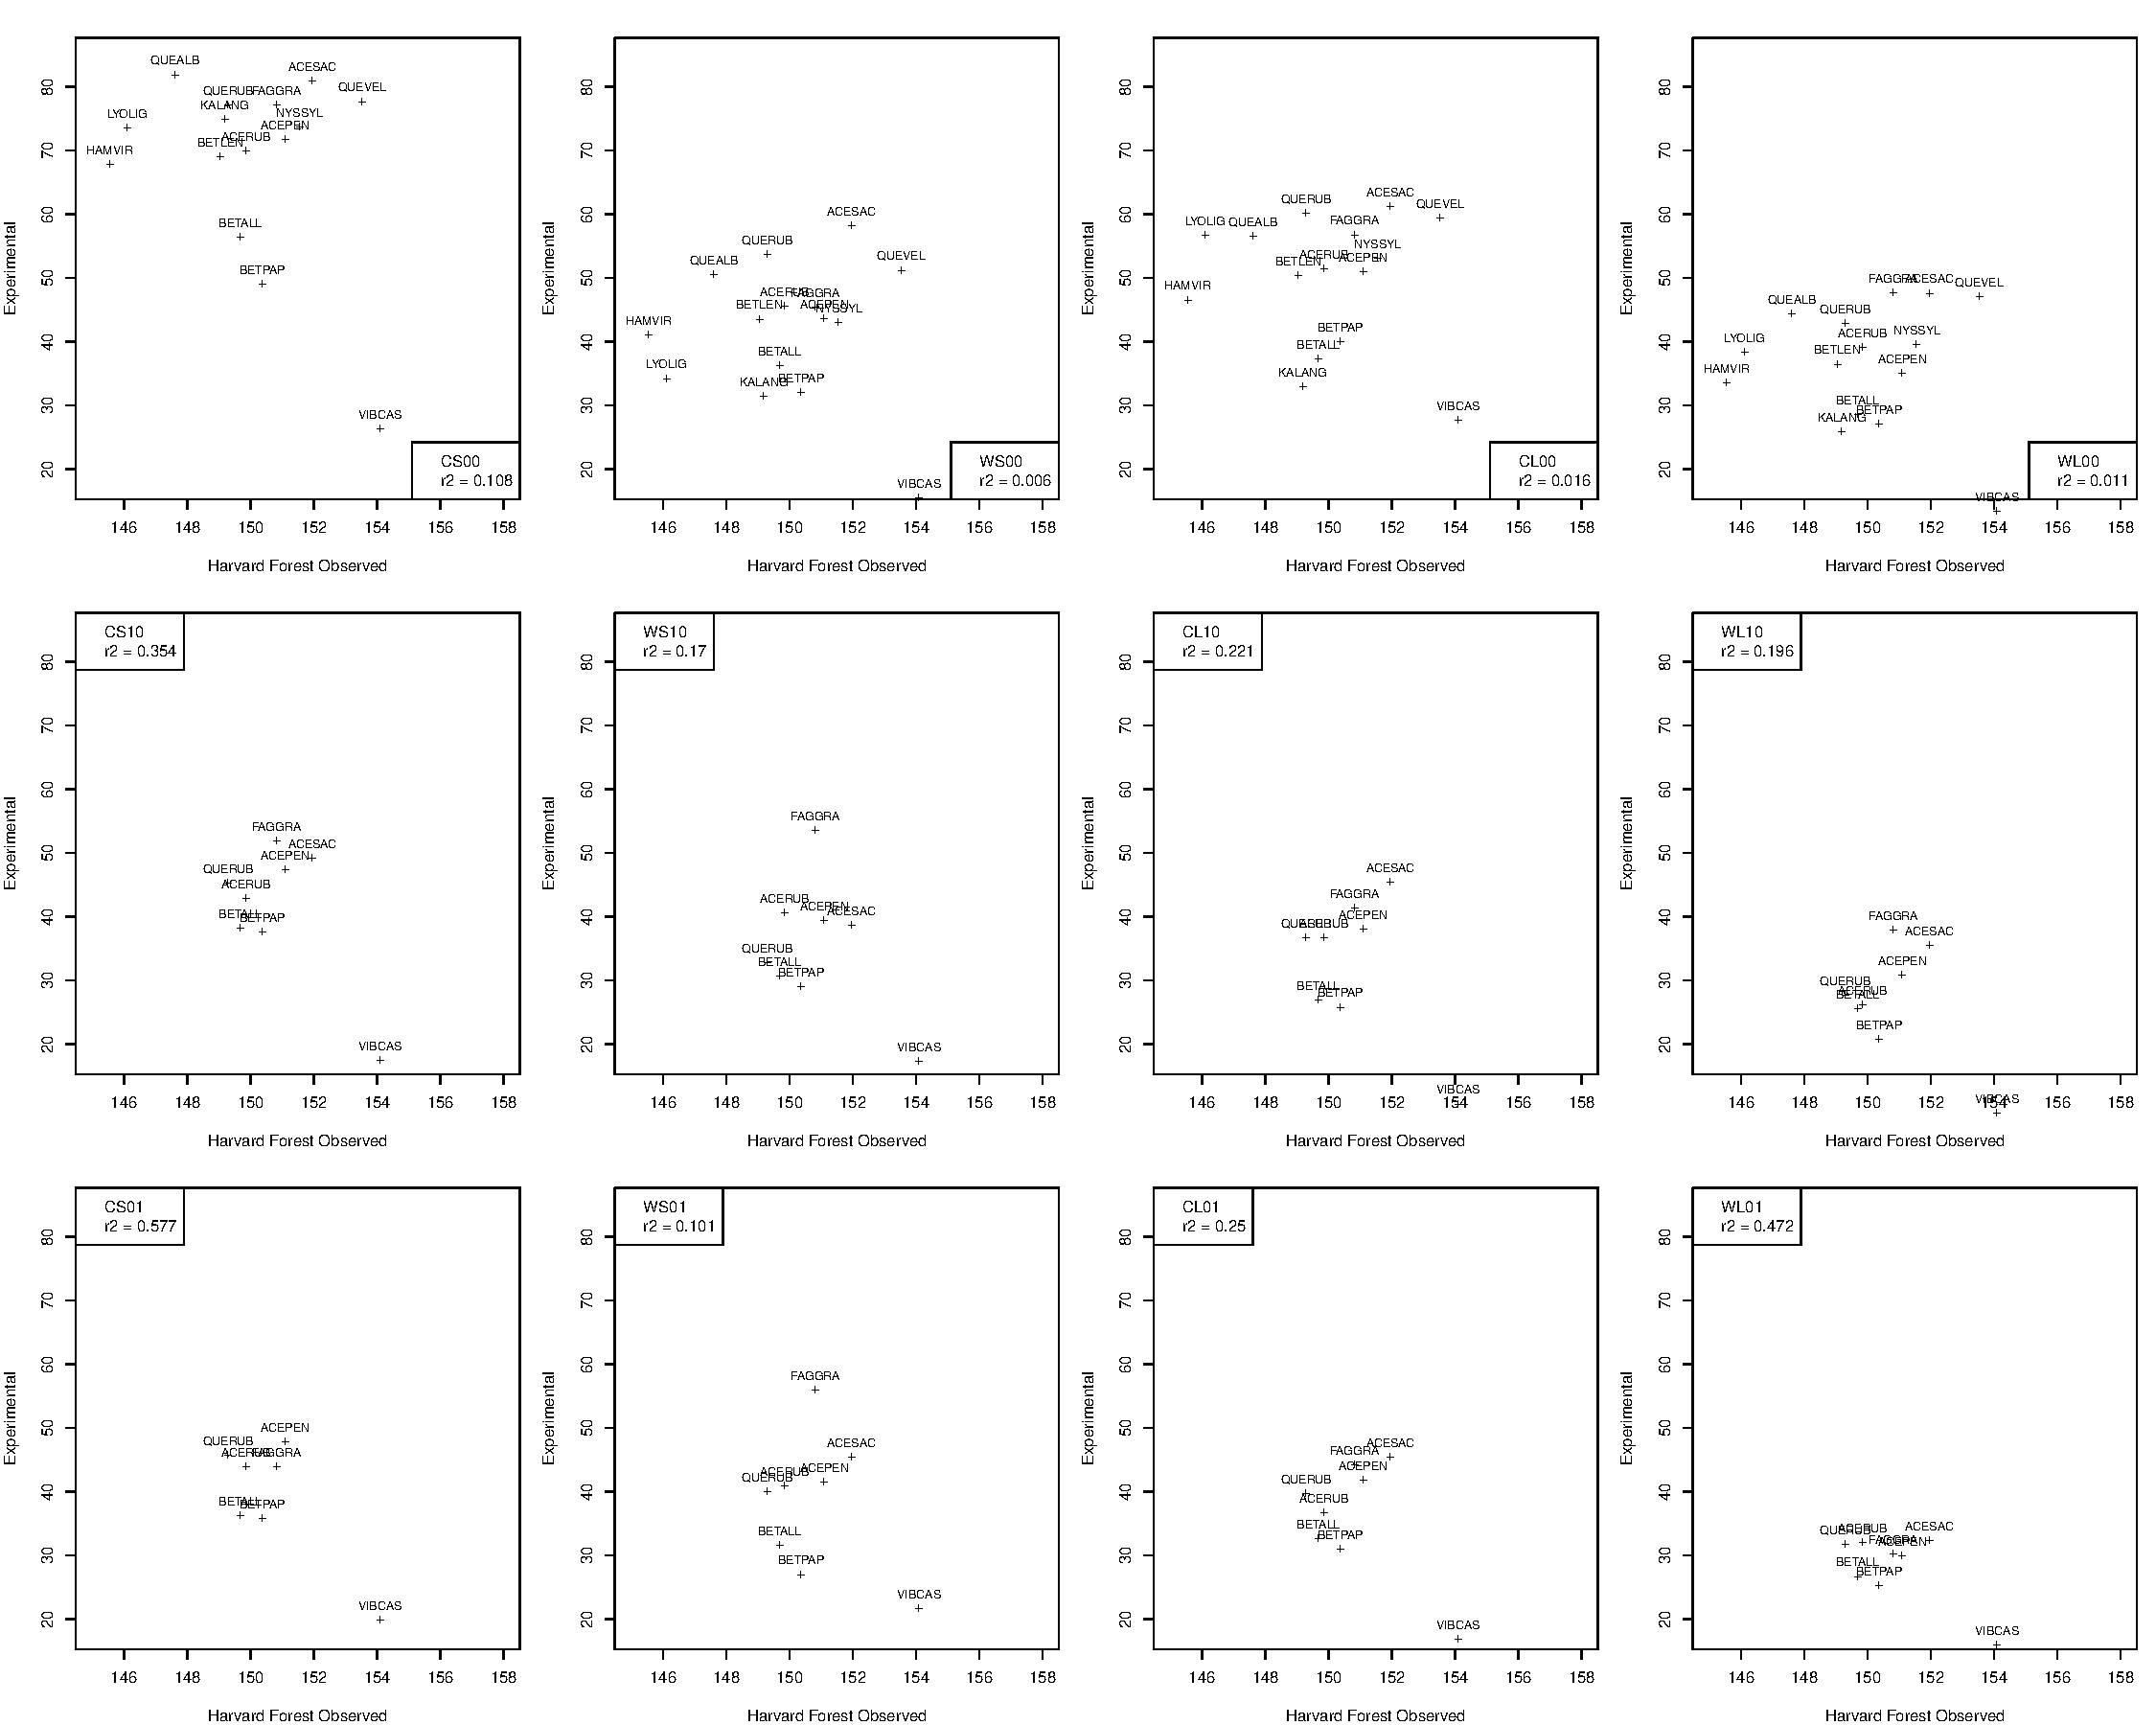
\includegraphics{leafout_exp_obs_corr_day}
\end{figure}


%\bibliography{/Users/danflynn/Dropbox/References/Bibrefs/danlib}
%\bibliographystyle{naturemag}

\end{document}
